\documentclass{new-aiaa}
\usepackage[utf8]{inputenc}
\usepackage{graphicx}
\usepackage{amsmath}
\usepackage{siunitx}
\usepackage{hyperref}
\usepackage{booktabs}
\usepackage{amssymb}
\usepackage{float}

\title{Design, Simulation, and Testing of a Modular Cold Gas Thruster System for CubeSat Applications}

\author{Jaxsen Cheeks \thanks{Undergraduate Student, School of Aerospace Engineering, Georgia Institute of Technology, Atlanta, GA.}}

\begin{document}
\maketitle

\begin{abstract}
Cold gas propulsion systems offer a simple, reliable, and low-cost solution for small satellite maneuvering and attitude control. Utilizing pressurized inert gases such as carbon dioxide or nitrogen, these systems provide limited but highly controlled thrust, making them ideal for CubeSats and nanosatellites operating in low Earth orbit. This paper presents the design, simulation, and testing of a benchtop cold gas thruster system with an accompanying simulation toolkit, CAD design, and a literature-informed proposal, drawing inspiration from current academic and industrial advancements.
\end{abstract}

\section*{Nomenclature}
\begin{tabbing}
    $P_0$ \quad \= Stagnation (regulated input) pressure (Pa) \\
    $P_a$ \> Ambient pressure (Pa) \\
    $T_0$ \> Stagnation (input) temperature (K) \\
    $\gamma$ \> Specific heat ratio (isentropic exponent) \\
    $R$ \> Specific gas constant (J/kg$\cdot$K) \\
    $C_d$ \> Discharge coefficient \\
    $A_t$ \> Nozzle throat area (m$^2$) \\
    $d_t$ \> Nozzle throat diameter (m) \\
    $d_e$ \> Nozzle exit diameter (m) \\
    $A_e$ \> Nozzle exit area (m$^2$) \\
    $\dot{m}$ \> Mass flow rate (kg/s) \\
    $v_e$ \> Exhaust velocity (m/s) \\
    $F$ \> Thrust (N) \\
    $I_{sp}$ \> Specific impulse (s) \\
\end{tabbing}


\section{Introduction}

In recent years, the use of CubeSats and small satellites has grown rapidly due to their cost-effectiveness and versatility. Their smaller volume and lower costs both contribute to a simple equation that benefits industry giants and emerging ventures alike. Smallsats serve a wide range of purposes, including environmental data collection, telecommunications, and technological demonstrations, with operators hailing from academia, government agencies, and commercial enterprises. However, because these satellites are designed to be more compact than their traditional counterparts, manufacturers face significant constraints when adding subsystems beyond the satellite’s primary mission.

One of the major challenges for smallsat platforms is the development of reliable, efficient, and compact propulsion systems. Historically, many CubeSat missions opted out of incorporating propulsion, relying instead on deployment mechanisms or passive orbital decay. However, as mission complexity increases, the need for precise maneuvering, station keeping, and deorbiting has grown. Traditional propulsion systems, such as chemical and electric thrusters, provide high performance but are often unsuitable for CubeSats due to their complexity, cost, and safety concerns. Cold gas propulsion systems offer a promising alternative due to their simplicity, operational safety, and low cost, although they deliver lower performance than chemical or electric systems.

This paper presents the design, simulation, and testing of a modular benchtop cold gas thruster system developed as a proof of concept for CubeSat-scale propulsion applications. The project integrates hardware prototyping, CAD modeling, and a simulation toolkit using MATLAB and Python to predict system performance. Drawing inspiration from recent research by NASA and the Georgia Tech Space Systems Design Lab (SSDL), this work aims to demonstrate the feasibility of a compact, reliable, and low-cost propulsion solution for future small satellite missions.


\section{Background and Literature Review}

Cold gas propulsion systems use stored, pressurized inert gaseous or liquid propellant expelled through a nozzle to generate thrust. This process leverages the principle of isentropic expansion, where gas accelerates through the nozzle by converting potential energy (pressure) into kinetic energy (thrust) with no heat transfer and constant entropy \cite{nasa2021}. The nozzle geometry, particularly the throat and expansion ratio, plays a critical role in determining flow efficiency and performance. When the flow reaches sonic conditions (Mach 1) at the nozzle throat, it becomes choked, meaning the mass flow rate depends solely on upstream pressure and nozzle dimensions, ensuring predictable thrust output even in varying space conditions. 
\begin{figure}[h!]
    \centering
    \includegraphics[width=0.7\textwidth]{images/cold gas principles.png}
    \caption{Simplified nozzle diagram illustrating isentropic expansion and choked flow in a cold gas propulsion system.}
    \label{fig:nozzle}
\end{figure}

The simplicity of cold gas systems stems from their reliance on a single propellant fluid, eliminating the need for complex fuel-oxidizer systems or extensive power storage required by traditional chemical or electric propulsion \cite{nasa2021}. These characteristics result in propulsion solutions that are lighter, less complex, and more cost-effective, making them particularly attractive for CubeSat and small satellite missions constrained by mass, volume, and budget. Such systems are often chosen by universities, research institutions, and organizations developing exploratory or educational missions. However, cold gas systems do have inherent limitations, including lower specific impulse (typically 50–70 seconds), low thrust levels (on the order of millinewtons), and limited delta-v capacity \cite{khader2018space}.

Within recent years, studies from NASA \cite{nasa2021}, Khader et al. \cite{khader2018space}, and the Georgia Tech Space Systems Design Lab (SSDL) \cite{skidmore2016}-among others- have established a strong foundation for cold gas propulsion systems in small satellite missions. NASA's comprehensive report on small satellite propulsion systems highlights cold gas thrusters as a viable and reliable option for both altitude control and minor orbital maneuvers, emphasizing their simplicity and low complexity \cite{nasa2021}. Khader et al. provide a detailed review of micropropulsion technologies for CubeSats and small satellites, discussing cold gas thrusters alongside alternatives like resistojet and electric propulsion systems \cite{khader2018space}. Their work emphasizes cold gas systems' operational simplicity and safety, while acknowledging limitations in specific impulse and thrust permormance. Georgia Tech's SSDL has demonstrated a CubeSat-scale cold gas system for the SunRISE mission, featuring moduler design, Arduino-based control, and the use of krypton as its propellant \cite{skidmore2016}. Together, these studies provide a comprehensive background to support the exploration of this project. 

Recent research has focused on advancing cold gas propulsion technology to address its inherent limitations and expand its capabilities for small satellite missions \cite{nasa2021,khader2018space,skidmore2016,adelis2019}. Additive manufacturing techniques, such as 3D printing, have enabled the fabrication of complex nozzle geometries, improving gas flow efficiency and system compactness \cite{skidmore2016}. Microelectromechanical systems (MEMS) have been explored to develop micro-thrusters with precise control and scalability, opening new possibilities for formation flying and distributed satellite architectures \cite{khader2018space}. Modular and plug-and-play propulsion systems, like those used in Adelis-SAMSON, have facilitated integration into diverse CubeSat platforms while reducing development time \cite{adelis2019}. Despite these innovations, cold gas systems remain limited by their low specific impulse and total impulse, constraining their use to attitude control and minor orbital adjustments \cite{nasa2021,khader2018space}. Future research is likely to focus on hybrid systems, improved propellant storage designs, and nozzle optimization to enhance performance while maintaining simplicity and safety \cite{nasa2021,khader2018space}.

This project builds upon these ongoing research efforts, drawing insights from NASA’s reports, the comprehensive review by Khader et al., and the Georgia Tech Space Systems Design Lab’s work. By integrating hardware prototyping, simulation modeling, and CAD design, this modular benchtop cold gas thruster system provides a practical demonstration platform for CubeSat-scale propulsion development. Additionally, the project offers educational value, serving as a practical, hands-on application of coursework and extracurricular knowledge.


\section{System Design}

The benchtop cold gas thruster system for this project is structured into five key subsystems: propellant and propellant storage, flow control, nozzle assembly, electronics and control logic, and system mounting with integrated safety measures. The following subsections outline each component's design considerations and implementation.

\subsection{Propellant and Storage System}
\subsubsection{Propellant Choice}
The propellant selected for this cold gas thruster system is carbon dioxide (CO$_2$), chosen for its safety, availability, and ease of use, especially for a student-level. Given the constraints of limited manufacturing capabilities, budget considerations, and reliance on consumer-accessible products, the choice prioritized safety and simplicity. Non-flammable, low-toxicity propellants such as R-134a and CO$_2$ emerged as ideal candidates, with CO$_2$ being widely available through consumer-grade sources like SodaStream and paintball cartridges. These options provide a balance of affordability (R-134a: $\sim\$10$–30; CO$_2$: $\sim\$10$–50) and compatibility with readily available tanks and valves \cite{nasa2021,khader2018space,skidmore2016}. While compressed air offers the safest and simplest approach, its lower performance limits its suitability for propulsion testing. Higher-performance but flammable options such as butane and propane were considered but ultimately rejected due to safety concerns, particularly in a home setting. This rationale highlights the trade-offs made to achieve a safe, functional, and cost-effective cold gas propulsion system for student-level experimentation.


\begin{table}[h!]
\centering
\caption{Cold Gas Propellant Candidates for Home Builds}
\begin{tabular}{@{}llllll@{}}
\toprule
\textbf{Propellant} & \textbf{Safety} & \textbf{Availability} & \textbf{Complexity} & \textbf{Cost} \\ \midrule
\textbf{R-134a} & Non-flammable &  Auto AC refrigerant & Simple & \$10--30 \\
\textbf{CO$_2$} &  Non-flammable, inert &  SodaStream, paintball & Simple (adapters) & \$10--50 \\
\textbf{Compressed Air} &  Safe &  Air compressor/tanks & Simple & Very low\\
\textbf{Butane} &  Flammable &  Camping canisters & Low (adapters) & \$3--10\\
\textbf{Propane} &  Flammable &  Camping tanks & Moderate & \$10--20 \\
\textbf{Nitrogen (N$_2$)} &  Inert, safe &  Welding suppliers & Moderate & \$50--100 \\
\bottomrule
\end{tabular}
\end{table}


\subsubsection{Propellant Storage Tank}
The cold gas system utilizes a commercially available 12oz CO$_2$ paintball tank. This type of tank was selected due to its widespread availability, ease of handling, and compatibility with common regulators and consumer-grade hardware. The tank is safety-certified (DOT, CE) for high-pressure gas storage and is designed to handle approximately 800 psi (55 bar) at room temperature. Its built-in regulator and standardized fittings ensure safe and convenient integration into the propulsion system, while providing sufficient volume for experimental cold gas propulsion tests.

\subsubsection{Pressure Regulator}
A commercially available, adjustable paintball CO$_2$ regulator was selected for the system. This regulator is designed for use with 12oz CO$_2$ paintball tanks and supports an output pressure range of 0–300 psi. For safe testing and controlled propellant flow, the regulator output is set to approximately 50–100 psi. This range provides sufficient thrust for experimental propulsion tests while ensuring low-pressure, safe operating conditions. The regulator is widely available through online retailers and sporting goods stores and is compatible with the paintball tank's standard CGA 320 thread, ensuring a secure and reliable connection.

\subsubsection{Tubing and Fittings}

The tubing selected for the system is PTFE (Teflon), chosen for its excellent chemical resistance, smooth internal surface, and moderate pressure capability suitable for CO$_2$ use. The tubing has a 1/4" outer diameter (OD), providing a balance of flexibility, flow capacity, and ease of handling. Compression fittings made of brass or stainless steel are used to secure the tubing, ensuring a reliable and leak-free connection under system pressure. Both the PTFE tubing and compression fittings are rated for pressures well above the system's nominal operating range of 50–100 psi, offering a significant safety margin.

\subsection{Flow Control Subsystem}

The flow control subsystem incorporates a 12V DC solenoid valve rated for moderate pressures (up to 100 psi), selected for its compatibility with CO$_2$ and commercial availability. The valve is actuated by an Arduino microcontroller through a logic-level N-channel MOSFET switch, allowing precise control of firing duration and system operation. A 12V DC power supply provides power to the solenoid valve, while the Arduino is powered separately via USB or a dedicated 5V supply. A flyback diode is included across the solenoid terminals to protect the electronics from voltage spikes during valve deactivation. No pressure sensor is included in the flow path, as the system’s performance can be monitored through controlled regulator settings and propellant flow rates.


\subsection{Nozzle Design and Fabrication}

The nozzle used in this cold gas propulsion system is a converging–diverging (C–D) nozzle, designed to facilitate efficient expansion of CO$_2$ gas. The geometry consists of a smooth converging section leading to a narrow throat (2 mm diameter), followed by a diverging exit (4 mm diameter). This configuration is based on classical compressible flow theory and enables the flow to reach Mach 1 at the throat under choked conditions, with potential for supersonic expansion in the diverging section if pressure conditions allow.

The design calculations assume isentropic flow and ideal gas behavior. The nozzle was modeled using SolidWorks and fabricated via 3D printing using high-strength PETG, chosen for its durability and chemical resistance.

\vspace{0.5em}
\noindent
\textbf{Design Parameters (Table~\ref{tab:nozzleparams}):}

\begin{table}[h]
\centering
\caption{C–D Nozzle Design Parameters}
\label{tab:nozzleparams}
\begin{tabular}{ll}
\toprule
\textbf{Parameter} & \textbf{Value} \\
\midrule
Propellant & CO$_2$ \\
Chamber Pressure ($P_0$) & 50 psi $\approx$ 344,738 Pa \\
Ambient Pressure ($P_a$) & 1 atm = 101,325 Pa \\
Temperature ($T_0$) & 293 K \\
Specific Heat Ratio ($\gamma$) & 1.3 \\
Gas Constant for CO$_2$ ($R$) & 188.9 J/kg·K \\
Discharge Coefficient ($C_d$) & 0.9 \\
Throat Diameter & 2 mm \\
Exit Diameter & 4 mm \\
\bottomrule
\end{tabular}
\end{table}

\vspace{0.5em}
\noindent

\vspace{0.5em}
\noindent
The nozzle is mounted to the propulsion system using a compression fitting for 1/4" OD tubing. Post-processing steps such as sanding were applied to smooth the internal walls and reduce turbulence. This design allows for safe, testable cold gas expansion under ambient conditions, while approximating the performance of a space-bound cold gas thruster.


\subsubsection{Calculated Performance}
\noindent\textbf{Throat Area:}
\[
A_t = \pi r_t^2 = \pi (0.001)^2 = 3.14 \times 10^{-6} \ \text{m}^2
\]
\noindent\textbf{Mass Flow Rate:}
\[
\dot{m} = C_d A_t P_0 \sqrt{\frac{\gamma}{R T_0}} \left( \frac{2}{\gamma+1} \right)^{\frac{\gamma+1}{2(\gamma-1)}} \approx 5.08 \times 10^{-4} \ \text{kg/s}
\]
\noindent\textbf{Exhaust Velocity:}
\[
v_e = \sqrt{\frac{2 \gamma R T_0}{\gamma - 1}} \approx 693 \ \text{m/s}
\]
\noindent\textbf{Thrust:}
\[
F = \dot{m} v_e \approx 0.353 \ \text{N}
\]
\noindent\textbf{Specific Impulse:}
\[
I_{sp} = \frac{F}{\dot{m} g_0} \approx 70.8 \ \text{s}
\]

\subsubsection{Modeling}
The nozzle geometry was modeled in SolidWorks, defining the throat and exit diameters with a smooth converging contour to minimize flow separation and turbulence. Fabrication was performed using a Prusa i3 MK3 3D printer, with PETG selected for its resistance to CO$_2$, durability, and moderate pressure capacity. Post-processing (light sanding) was applied to smooth internal surfaces and enhance flow characteristics. The nozzle is connected to the system using a brass compression fitting for 1/4" OD tubing, ensuring a secure, leak-free interface with the solenoid valve output.



\subsection{Microcontroller and Electronics Control}

The propulsion system’s electronics are controlled by an Arduino Uno microcontroller, which serves as the central unit for actuating the solenoid valve. A digital output pin from the Arduino switches a logic-level N-channel MOSFET (e.g., IRLZ44N), controlling the 12V power supply to the valve and enabling precise actuation based on Arduino logic. Pulse timing for the solenoid valve is implemented via Arduino code, regulating firing duration to control propellant flow during tests.

Power is provided by a 12V DC supply (e.g., wall adapter or battery pack) for the solenoid valve and a separate USB or 5V DC supply for the Arduino, ensuring isolated control and actuation circuits. Protective components include a flyback diode (e.g., 1N4007) across the solenoid terminals to prevent voltage spikes caused by coil deactivation, and an optional current-limiting resistor in the MOSFET gate connection for signal conditioning, though the Arduino’s digital pin typically drives the MOSFET gate directly.

The circuit is initially assembled on a breadboard for prototyping and testing, with plans to transition to a more durable protoboard after validation. This approach provides safe, reliable, and adjustable operation of the cold gas propulsion system using standard, readily available components and prototyping methods.


\subsection{System Mounting and Safety Measures}

All system components will be mounted on a rigid plywood baseplate, manufactured to accommodate the system layout and provide easy access for assembly and testing. Components will be securely fixed to the baseplate using a combination of metal brackets, hose clamps, and zip ties to prevent movement during operation. Compression fittings will be used for tubing connections, ensuring leak-free seals and robust mechanical connections. Key components, including the solenoid valve and regulator, will be anchored directly to the baseplate to minimize vibrations and the risk of accidental disconnections.

Safety measures incorporated into the system include a pressure relief valve or pre-set regulator to ensure system pressure does not exceed the rated limits of the tubing and components (nominally 100 psi). Testing will be conducted in a controlled, outdoor workspace, clear of flammable materials and with adequate ventilation. Appropriate personal protective equipment (PPE), including safety glasses and gloves, will be used during all assembly and testing operations to mitigate potential hazards. These measures collectively ensure safe and reliable operation of the cold gas propulsion system under test conditions.

\subsection{System Architecture}

To summarize the complete cold gas propulsion system architecture, a Piping and Instrumentation Diagram (P\&ID) is provided in Figure~\ref{fig:pid}. This schematic integrates all major components discussed in the previous sections, including the propellant tank (PT-01), regulator (PPR-01), solenoid valve (PPV-01), control electronics (CTRL-01), and nozzle (N-01). The diagram also includes key safety features such as a pressure relief valve (PRV-01) and in-line pressure monitoring (PG-01), as well as the power supply interfaces (PS-01 and PS-02).

The P\&ID illustrates both fluid flow (CO$_2$) and electrical control pathways, highlighting how each subsystem interconnects during operation. Control signals from the microcontroller actuate the solenoid valve to regulate thrust, while regulated CO$_2$ flows from the tank through the valve and nozzle to generate impulse. The full component tag legend is provided in Table~\ref{tab:pid-legend}.



\begin{figure}[H]
\centering
\begin{minipage}{0.7\textheight}
    \centering
    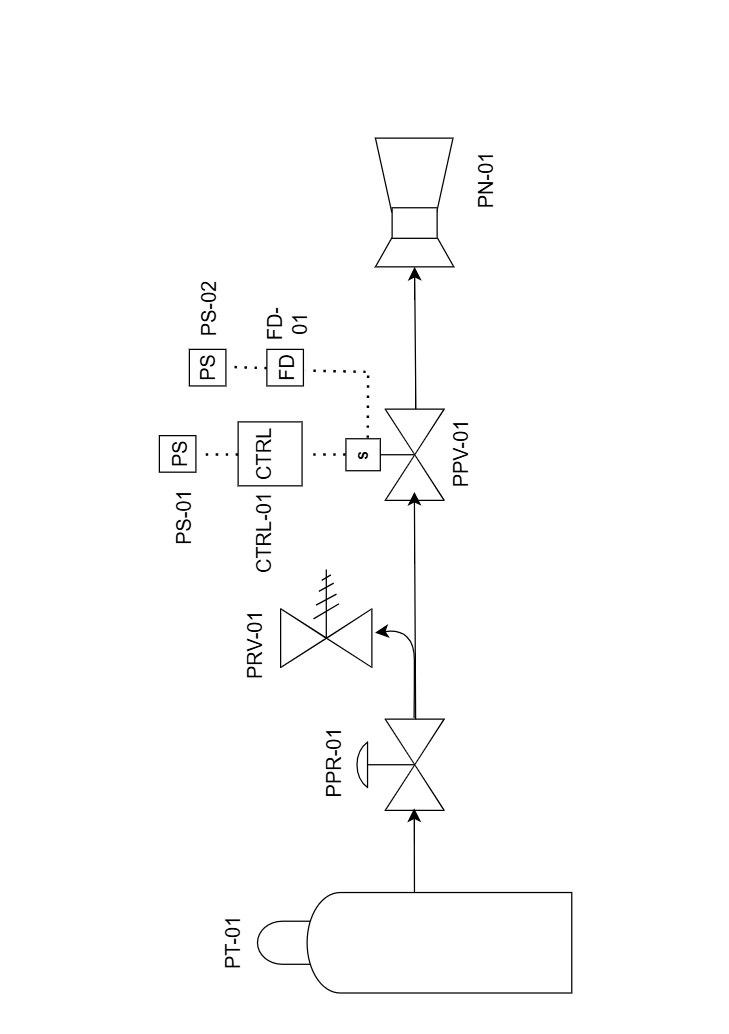
\includegraphics[height=0.9\textwidth,angle=270]{images/CG-PID-v1.png} 
    \caption{Piping and Instrumentation Diagram (P\&ID) for the cold gas propulsion system.}
    \label{fig:pid}
\end{minipage}
\hfill
\begin{minipage}{0.45\textheight}
    \centering
    \captionof{table}{P\&ID Component Legend}
    \begin{tabular}{lll}
        \toprule
        \textbf{Tag} & \textbf{Component} & \textbf{Notes} \\
        \midrule
        PT-01 & CO$_2$ Tank & 12oz, 800 psi \\
        PPR-01 & Regulator & 50–100 psi output \\
        PRV-01 & Pressure Relief Valve & Cracks at ~100 psi \\
        PPV-01 & Solenoid Valve (NC) & 12V, Arduino controlled \\
        CTRL-01 & Microcontroller & Arduino Uno \\
        FD-01 & Flyback Diode & 1N4007 \\
        PS-01 & Power Supply & 12V for solenoid \\
        PS-02 & Power Supply & USB/5V for Arduino \\
        PG-01 & Pressure Gauge & Upstream of nozzle \\
        PN-01 & Nozzle & 2 mm throat, 4 mm exit \\
        \bottomrule
    \end{tabular}
    \label{tab:pid-legend}
\end{minipage}
\end{figure}




\section{Integration and Testing}

\subsection{System Assembly}
The system assembly follows a structured order of operations:
\begin{enumerate}
    \item Mount the plywood baseplate and attach all components, including the CO$_2$ tank, regulator, solenoid valve, tubing, and nozzle.
    \item Secure tubing connections using compression fittings and clamps.
    \item Wire the Arduino, MOSFET, solenoid valve, and protective components on a breadboard.
    \item Connect power supplies: 12V for the solenoid valve, and USB or 5V for the Arduino.
    \item Perform pre-checks for wiring integrity and mechanical security, including:
    \begin{itemize}
        \item Verifying all fittings are properly tightened.
        \item Confirming correct wiring connections.
        \item Double-checking regulator pressure settings and valve orientation.
    \end{itemize}
\end{enumerate}

\subsection{Testing Procedures}
A series of tests will be conducted to ensure system functionality and safety:
\begin{itemize}
    \item \textbf{Leak Test}: Apply soapy water or use a gas leak detector on all tubing and fittings prior to pressurization.
    \item \textbf{Valve Function Test}: Verify solenoid valve operation in response to Arduino commands at low pressure.
    \item \textbf{Nozzle Performance Test}: Observe and evaluate the CO$_2$ jet for thrust and flow characteristics.
    \item \textbf{Timing Test}: Measure valve response time and actuation duration controlled by Arduino timing functions.
\end{itemize}

\subsection{Performance Monitoring}
\begin{itemize}
    \item \textbf{Pressure Monitoring}: Use a pressure gauge upstream of the nozzle or monitor regulator output to confirm operating pressure.
    \item \textbf{Flow Observation}: Visually observe the nozzle’s exhaust plume during tests.
    \item \textbf{Timing Measurements}: Use a stopwatch or Arduino timing functions to measure valve open duration and response times.
\end{itemize}

\subsection{Safety Procedures}
Safety measures implemented during testing include:
\begin{itemize}
    \item Conducting tests in a well-ventilated, outdoor workspace free of flammable materials.
    \item Wearing safety glasses and gloves during all testing operations.
    \item Beginning with low-pressure testing before gradually increasing to full operating conditions.
    \item Being prepared to disconnect power or shut off the regulator in case of malfunction.
    \item Never leaving the system unattended while pressurized or during tests.
\end{itemize}

\section{Simulation Toolkit}

The system’s performance and design calculations were modeled using  \textbf{Python}. The simulation toolkit includes several key computational modules:

\subsubsection{Key Functions}
\begin{itemize}
    \item Isentropic flow calculations to determine choked flow conditions.
    \item Mass flow rate estimation based on throat area and regulator pressure.
    \item Exhaust velocity and specific impulse modeling.
    \item Thrust estimation derived from mass flow rate and exhaust velocity.
\end{itemize}

\subsubsection{Simulation Inputs}
\begin{itemize}
    \item Upstream regulated pressure ($P_0$), e.g., 50 or 100 psi.
    \item Ambient temperature ($T_0$), e.g., 293 K ( or whatever temp on test day is)
    \item Nozzle throat area ($A_t$:\[ 3.14 \times 10^{-6} \ \text{m}^2\]
    \item Gas properties for CO$_2$: specific gas constant ($R$) and heat ratio ($\gamma$).
\end{itemize}

\subsubsection{Simulation Outputs}
\begin{itemize}
    \item Mass flow rate ($\dot{m}$) in kg/s.
    \item Exhaust velocity ($v_e$) in m/s.
    \item Thrust ($F$) in N.
    \item Specific impulse ($I_{sp}$) in s.
    \item Flow condition: choked or un-choked.
\end{itemize}

\subsubsection{Validation}
Validation of the simulation outputs was conducted through:
\begin{itemize}
    \item Comparison with theoretical predictions from compressible flow equations.
    \item Cross-checking of calculated thrust and mass flow rates with experimental test data (e.g., valve timing tests, nozzle flow observations).
    \item Qualitative comparison of simulated nozzle performance (plume behavior) with actual observations from experimental tests.
\end{itemize}

This simulation toolkit provides an effective means to predict, analyze, and refine system performance both before and during experimental operations.



\section{Results and Discussion}
key findings from build and tests, simulation results vs real-world data, system performance analysis, and lessons learned

\section{Conclusion and Future Work}
summary of contributions, system performance, and potential extensions to hybrid or green propulsion systems, and integration with CubeSat missions
could expand into experimenting with nozzle variations; nozzle throat diameter, nozzle exit diameter, convergent(current) vs divergent-convergent vs divergent

\bibliographystyle{new-aiaa}
\bibliography{reportBib}

\end{document}
